\documentclass[12pt]{article} % Default font size is 12pt, it can be changed here
\usepackage{geometry} % Required to change the page size to A4
\usepackage{graphicx} % Required for including pictures
\usepackage{float} % Allows putting an [H] in \begin{figure} to specify the exact location of the figure
\usepackage{wrapfig} % Allows in-line images such as the example fish picture
\usepackage{amssymb}
\usepackage{url}
\usepackage{pdfpages}
\geometry{a4paper} % Set the page size to be A4 as opposed to the default US Letter
\graphicspath{{graphs/}{img/}} % Specifies the directory where pictures are stored
\linespread{1.2} % Line spacing

\begin{document}

%----------------------------------------------------------------------------------------
%	TITLE PAGE
%----------------------------------------------------------------------------------------
\begin{titlepage}

\newcommand{\HRule}{\rule{\linewidth}{0.5mm}} % Defines a new command for the horizontal lines, change thickness here

\center% Center everything on the page

\textsc{\LARGE Universit\`a di Trento}\\[0.8cm] % Name of your university/college
\textsc{\Large Corso HCI A.A. 2014--2015}\\[0.8cm] % Major heading such as course name
\textsc{\large Partecipatory Development}\\[1.5cm] % Minor heading such as course title

\HRule\\[0.8cm]
{\huge \bfseries Gestione delle labels di Github}\\[0.4cm] % Title of your document
\HRule\\[2cm]

\begin{minipage}{0.4\textwidth}
\begin{flushleft} \large
\begin{tabular}{ll}
Bortoli \textsc{Gianluca} & \makebox[2cm][r]{159993} \\
Brugnara \textsc{Martin} & \makebox[2cm][r]{157791} \\
Dellera \textsc{Andrea} & \makebox[2cm][r]{158365} \\
Hoxha \textsc{Fatbardha} & \makebox[2cm][r]{161003}
\end{tabular}
\end{flushleft}
\end{minipage}

\vfill % Fill the rest of the page with whitespace
{\large \today}\\[3cm] % Date, change the \today to a set date if you want to be precise
\end{titlepage}

%----------------------------------------------------------------------------------------
%	TABLE OF CONTENTS
%----------------------------------------------------------------------------------------
\tableofcontents % Include a table of contents

\newpage % Begins the essay on a new page instead of on the same page as the table of contents

\section{Introduzione}
Il primo obiettivo di questo progetto consiste nell'analizzare quali siano le principali barriere nella partecipazione ai progetti open source, che oggigiorno sono diventati sempre pi\`u numerosi e di una certa rilevanza, in alcuni casi addirittura a livello mondiale.\\
Il nostro interesse \`e ricaduto proprio in tali problematiche che affliggono questo tipo di progetti, dal momento che sono state ravvisate anche in prima persona durante il corso dei nostri studi.\\
Questo approfondimento deriva in parte anche dalla nostra propensione e dal nostro interesse per l'utilizzo di software open source durante la carriera universitaria e lavorativa.\\
Ci prefiggiamo come scopo finale di trovare e formulare una possibile soluzione al problema della gestione delle etichette su Github (la piattaforma principe per lo sviluppo open source), dal momento che essa \`e attualmente poco organica e talvolta gestita in modo poco funzionale, soprattutto in progetti di una certa complessit\`a e dimensione.\\
\vfill
\begin{center}
Tutto il materiale raccolto, i prototipi, i sorgenti di questo progetto ed un video di demo si possono trovare nel repository su Githuib al seguente link:\\
\textbf{\url{https://github.com/MartinBrugnara/HCI}}
\end{center}

\newpage

\section{Interviste}
Il primo passo per l'individuazione delle principali problematiche legate all'ambito della partecipazione ai progetti open source \`e stata fatta tramite delle interviste. Tale tipologia di ricerca si presta molto alla valutazione di barriere come queste, dal momento che l'intervistato non si sente limitato nell'esprimersi (come potrebbe risultare da un questionario a risposta multipla), ma al contempo non ha la percezione di dilungarsi troppo (come invece potrebbe accadere se viene posto un questionario a domanda aperta), il che potrebbe indurlo a non scrivere tutto ci\`o che effettivamente pensa.\\
Con il tramite dell'intervista ``faccia a faccia'' questi inconvenienti vengono meno: la persona si sente pi\`u libera di discutere con l'intervistatore che pone le domande e l'intervistato non si sente bloccato mentre sta rispondendo, non interrompendo cos\`\i\ il flusso delle idee (che \`e la parte essenziale dell'intera intervista).\\

\subsection{Traccia}
La traccia\footnote{\url{http://disi.unitn.it/~deangeli/homepage/lib/exe/fetch.php?media=teaching:hci:hci2014_2015:intervista_pd_motivazioni.pdf}} delle domande da porre durante l'intervista ci \`e stata fornita direttamente dalla dottoressa Bordin, poich\'e tale argomento non era ancora stato trattato a lezione nel momento in cui questa parte del progetto \`e stata avviata.\\
Essa prevedeva dei quesiti mirati principalmente a capire:
\begin{itemize}
\item se e quali software open source vengano utilizzati
\item se l'intervistato partecipi/abbia partecipato attivamente a tali progetti
\item quali siano le motivazioni che lo abbiano portato a farlo oppure no
\item cosa significhi \emph{partecipare} ad un progetto open source
\end{itemize}

\subsection{Analisi dei risultati}
Il campione oggetto dell'intervista si compone di 12 persone. Esso non \`e molto eterogeneo, come \`e possibile notare in Figura~\ref{fig:distribuzione}, poich\'e \`e stato pi\`u immediato intervistare delle persone all'interno del nostro corso di laurea piuttosto che di altri atenei o di lavoratori.

\begin{figure}[H]
\center{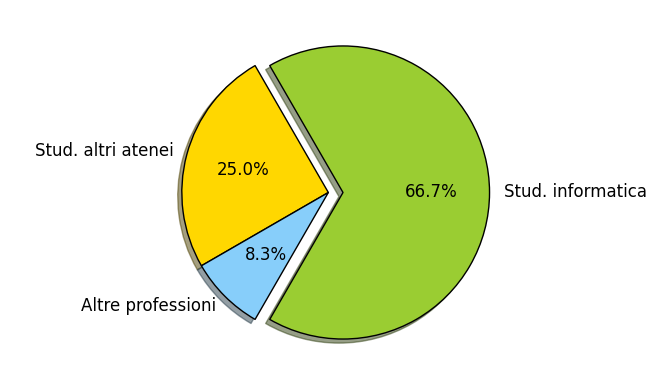
\includegraphics[width=0.8\linewidth]{interviewed_distribution.png}}
\caption{Distribuzione della professione delle persone intervistate.}
\label{fig:distribuzione}
\end{figure}

Abbiamo potuto notare come gli unici due intervistati che hanno contribuito attivamente a progetti open source provenissero esclusivamente da un ambito informatico. Inoltre, all'interno del gruppo stesso ben pochi lo hanno fatto, come \`e possibile notare dalla Figura~\ref{fig:distribuzioneInformatica}.

\begin{figure}[H]
\center{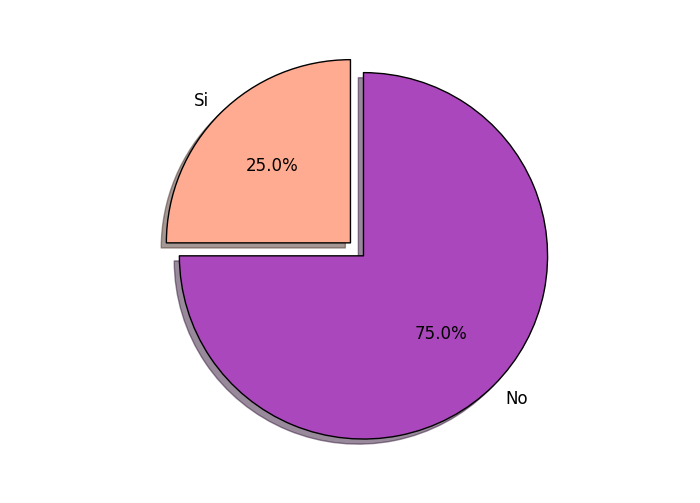
\includegraphics[width=0.8\linewidth]{interviewed_participation.png}}
\caption{Persone che hanno attivamente partecipato a progetti open source tra gli studenti di informatica.}
\label{fig:distribuzioneInformatica}
\end{figure}

Da ci\`o si deduce che l'ambito e la possibilit\`a di parteciparvi sono molto ristretti. Questi risultati ci permettono di delineare le caratteristiche della \emph{personas}, ovvero un personaggio fittizio con delle caratteristiche ben definite, che rappresentano il tipo di utente preso in considerazione (che possono esserpu\`o essere anche pi\`u di uno).\\
I tratti distintivi che abbiamo riscontrato a seguito delle interviste sono i seguenti:
\begin{itemize}
\item un consistente background informatico
\item un interesse verso il campo specifico del progetto considerato
\item tempo ed impegno da dedicarvi
\end{itemize}

In aggiunta abbiamo notato come lo \emph{scenario} accademico incentivi e contribuisca ad utilizzare specifici software open source e, di conseguenza, aumenti la probabilit\`a che uno studente si interessi e ne possa far parte.

\newpage

\section{Benchmarking}
Durante questa fase abbiamo scelto di concentrarci su tre progetti open source: NeoVim, CyanogenMod e OpenOffice.\\
Dopo averli presentati e descritti durante un workshop, abbiamo analizzato i pro ed i contro di ciascuno, da cui \`e emerso che molti utenti utilizzano spesso questi software sia per aspetti personali che in ambito lavorativo.\\
Quelli da noi considerati sono gratuiti\footnote{Bisogna porre attenzione a non confondere il concetto di open source con quello di freeware: Una licenza open source impone che il sorgente sia distribuito con il programma, ma non da indicazioni sul prezzo. Freeware, al contrario, prevede che non via sia costo d'acquisto, ma non regolamenta le modalita di distribuzione del sorgenete. (eg.\ RedHat \`e una distribuzione linux \emph{open source} la cui licenza \`e a pagamento\dots a partire da \$300)}, di facile utilizzo e mantenuti costantemente aggiornati dalla comunit\`a di sviluppo.\\
Inoltre le funzionalit\`a offerte sono molto simili a quelle dei rispettivi software equivalenti, se non addirittura meglio sviluppate.\\
Al contrario, essi non vengono largamente utilizzati a causa della ridotta conoscenza del prodotto, dal momento che vengono scarsamente pubblicizzati, e per la loro intuitivit\`a di utilizzo, alla quale non si presta molta attenzione e sulla quale spesso non viene fatto uno studio molto approfondito.\\

\subsection{Contribuire ad un progetto}
\label{motivi}
Dalle interviste \`e emerso che il significato attribuito al termine \emph{contribuire} \`e, quasi all'unanimit\`a, quello di mettere a disposizione le proprie competenze per il miglioramento di un software e/o la risoluzione di eventuali problemi legati ad esso.\\
Le motivazioni che possono spingere a contribuire sono molte: dalla semplice soddisfazione per aver risolto un bug, all'arricchimento personale e l'esperienza acquisita che ne consegue, passando per la necessit\`a di dover implementare una funzionalit\`a che risolva un problema che ci si trova a fronteggiare durante il proprio lavoro.\\
Al contrario, altrettanti sono i motivi che portano, invece, le persone a non contribuire, tra i quali la mancanza di tempo e di competenze, ma soprattutto la \emph{qualit\`a} e disponibilit\`a delle \emph{informazioni} riguardanti un progetto.\\
Quest'ultimo a nostro avviso risulta essere il pi\`u rilevante, dal momento che un utente (con delle capacit\`a per farlo) si trova a non poter contribuire a causa della mancanza di linee guida su come realizzarlo. Ci\`o potrebbe sembrare banale a primo impatto, ma \`e una costante in molti dei progetti presi in considerazione.

\newpage

\section{Design library: NeoVim}
Nella nostra \emph{design library} ci siamo concentrati sul progetto di NeoVim per poter individuare sia degli esempi sia di buona che di cattiva progettazione da cui prendere spunto.\\

\subsection{Buoni esempi}
Delineeremo ora una lista degli esempi pi\`u significativi di un design pensato e studiato appositamente per far s\`\i\ che l'utente interessato a partecipare riesca a farlo nel modo migliore possibile.\\
Abbiamo notato come sia il sito di NeoVim che la gestione della codebase su Github siano state progettate secondo il paradigma dell'\emph{user driven design}, il quale mira a massimizzare la fruibilit\`a del prodotto.

\begin{figure}[H]
\center{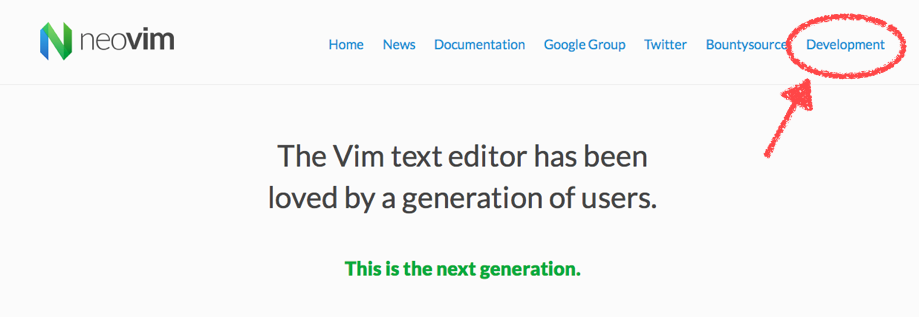
\includegraphics[width=0.8\linewidth]{buonesempio1.png}}
\caption{Homepage di NeoVim.}
\label{fig:buonesempio1}
\end{figure}

Dalla Figura~\ref{fig:buonesempio1} si pu\`o notare come il gruppo di sviluppo del progetto preso in considerazione indichi chiaramente nella pagina principale una sezione per chi volesse contribuire. Gi\`a da questo possiamo capire come si miri allo sviluppo di terzi: per questo motivo il link al codice sorgente del software su Github viene messo nel menu principale, in modo che sia di facile reperibilit\`a.

\begin{figure}[H]
\center{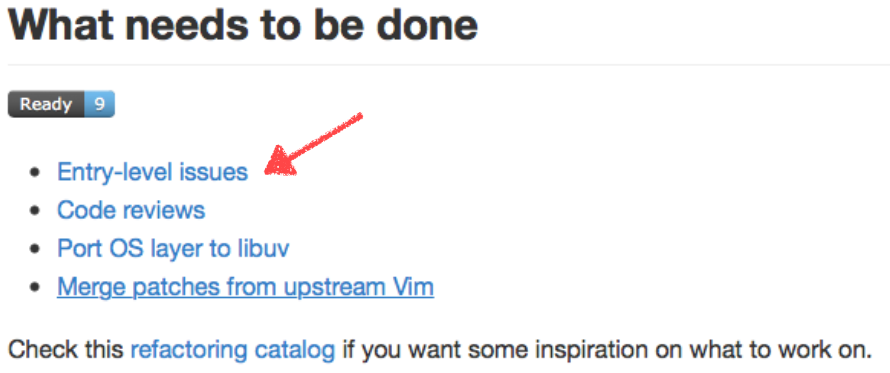
\includegraphics[width=0.65\linewidth]{buonesempio2.png}}
\caption{Cosa c'\'e da fare.}
\label{fig:buonesempio2}
\end{figure}

Un'altra criticit\`a riscontrata durante la fase di benchmarking \`e quella che il soggetto non ritenga di avere le capacit\`a sufficienti per dare il proprio contributo.\\
Ci\`o \`e stato parzialmente risolto (Figura~\ref{fig:buonesempio2}) introducendo dei \emph{livelli di difficolt\`a} per le issues/bug presenti nel software. \`E stata introdotta un'etichetta per i problemi di facile risoluzione (entry level issues), cosa che non avevamo mai notato prima negli altri progetti da noi presi in considerazione.

\begin{figure}[H]
\center{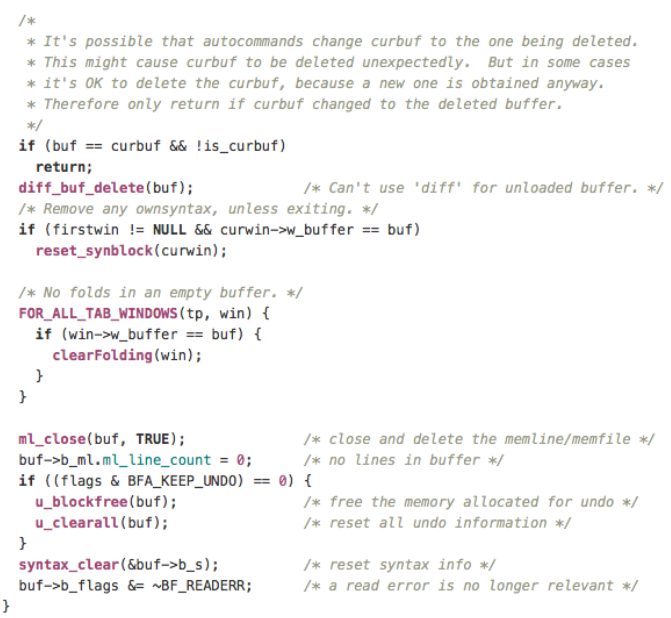
\includegraphics[width=0.65\linewidth]{buonesempio3.png}}
\caption{Homepage di NeoVim.}
\label{fig:buonesempio3}
\end{figure}

Infine, viene posta molta cura nella documentazione e nei commenti all'interno del codice. Ci\`o aiuta chi interviene in quella porzione di sorgente a poter capire meglio e senza eccessiva difficolt\`a cosa faccia una certa porzione di codice.\\
Inoltre, alla nascita di NeoVim, sono state decise delle linee guida ben precise su come si dovesse indentare/organizzare il codice e soprattutto su come commentarlo, in modo da non creare disomogeneit\`a all'interno del progetto (il che creerebbe sicuramente problemi di comprensione).\\

\subsection{Cattivi esempi}
\label{badexamples}
Allo stesso tempo abbiamo individuato delle parti che risultavano poco intuitive e che potevano creare delle difficolt\`a a chi volesse interagire.

\begin{figure}[H]
\center{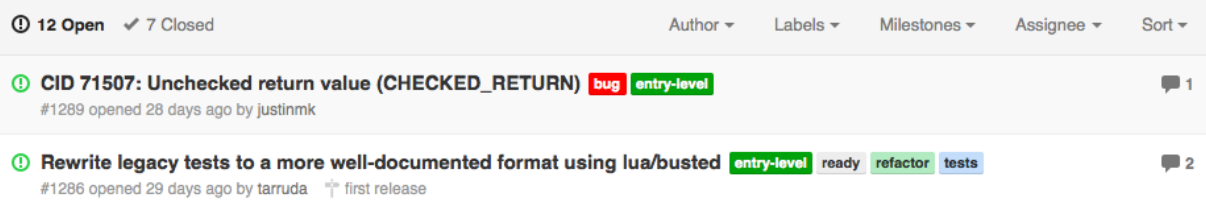
\includegraphics[width=0.65\linewidth]{cattivoesempio1.png}}
\caption{Etichette assegnate alle issue su Github.}
\label{fig:cattivoesempio1}
\end{figure}

Dalla Figura~\ref{fig:cattivoesempio1} gi\`a ad un primo impatto si pu\`o notare come le etichette assegnate alle issue ancora da risolvere siano poco esplicative e, a volte, ridondanti.\\
Questa situazione crea molta confusione nel momento in cui lo sviluppatore vuole dare il proprio contributo e, controllando cosa ci sia da fare e/o correggere, si trova davanti ad una un'infinit\`a di labels con i colori pi\`u disparati e visualizzate in modo disorganizzato e poco coerente.

\begin{figure}[H]
\center{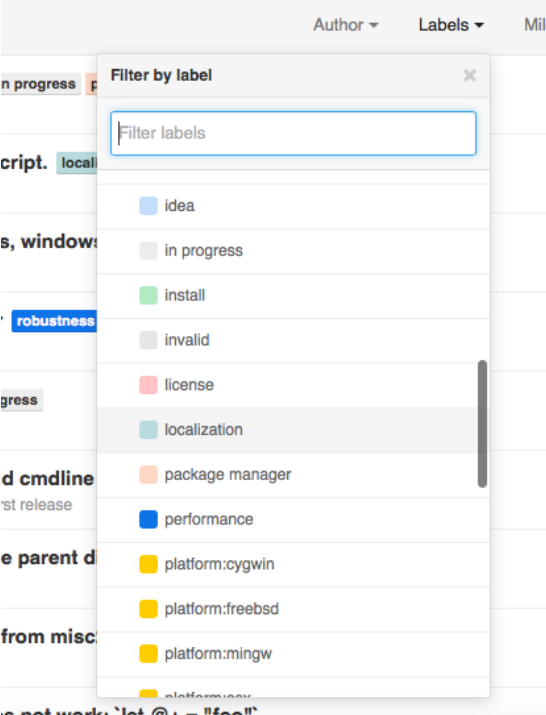
\includegraphics[width=0.4\linewidth]{cattivoesempio2.png}}
\caption{Menu per la selezione delle labels.}
\label{fig:cattivoesempio2}
\end{figure}

Quello della coerenza e dei colori diventa ancora pi\`u problematico nel momento in cui si vuole filtrare per label tutte le issue.\\
A colori molto simili e talvolta identici sono associate delle problematiche e delle aree di lavoro molto differenti tra loro. Come si pu\`o vedere dalla Figura~\ref{fig:cattivoesempio2}, le voci \emph{licence} e \emph{package manager} hanno una colorazione quasi indistinguibile, nonostante riguardino due ambiti molto diversi.

\begin{figure}[H]
\center{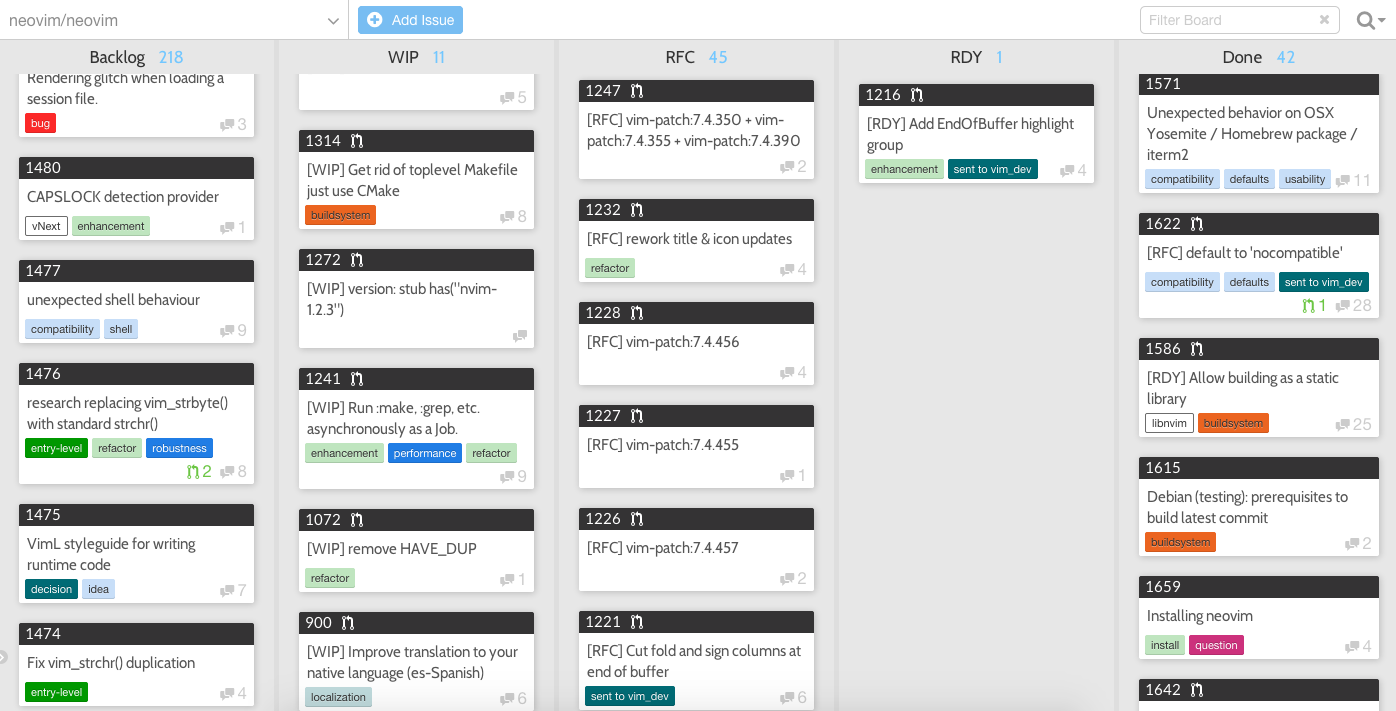
\includegraphics[width=0.8\linewidth]{cattivoesempio3.png}}
\caption{Homepage di NeoVim.}
\label{fig:cattivoesempio3}
\end{figure}

Il problema si estende anche a \emph{Waffle}\footnote{\url{www.waffle.io}}, un tool che permette di gestire in modo pi\`u comodo ed immediato le issues di Github in tempo reale. Grazie a questo software direttamente collegato a Github non c'\'e la necessit\`a di controllare manualmente lo stato attuale del lavoro, bens\`\i\ viene organizzato automaticamente in base ai commit e alle issue a cui fanno riferimento.\\
Dalla Figura~\ref{fig:cattivoesempio3} si evince che la visualizzazione del flusso di lavoro viene intaccata e resa di difficile comprensione a causa della cattiva gestione delle labels.

\newpage

\section{Prototipi}
Considerando gli esempi raccolti nella design library, avendo visionato i risultati ottenuti dalle interviste e dopo aver identificato quali siano le problematiche che ostacolano maggiormente la partecipazione ai progetti open source, abbiamo deciso di porre particolare attenzione alla gestione delle labels su Github.\\
Il lavoro da noi svolto ha come punto di riferimento ci\`o che abbiamo potuto osservare all'interno del progetto di NeoVim.\\

\subsection{Prototipo a bassa fedelt\`a}
Utilizzando \emph{Balsamiq\footnote{\url{www.balsamiq.com}}} abbiamo realizzato un primo prototipo a bassa fedelt\`a.\\
Le label che fanno riferimento a problemi della stessa area vengono raggruppate in una singola macro-label, espandibile con un click. L'idea \`e quella di implementare il \emph{design pattern} file-cartella.\\
Dopo aver riflettuto a fondo, abbiamo deciso di limitare ad un solo livello la profondit\`a raggiungibile dalla struttura gerarchica delle labels. Ci\`o significa che se un'etichetta appartiene gi\`a ad una macro-label, essa non pu\`o avere ulteriori sotto-label che creino un altro sottoalbero.\\
Questa decisione, per quanto inizialmente potesse sembrare una limitazione nei confronti dell'utente finale, aiuta a mantenere la semplicit\`a e la praticit\`a delle label senza introdurre difficolt\`a di utilizzo.

\begin{figure}[H]
\center{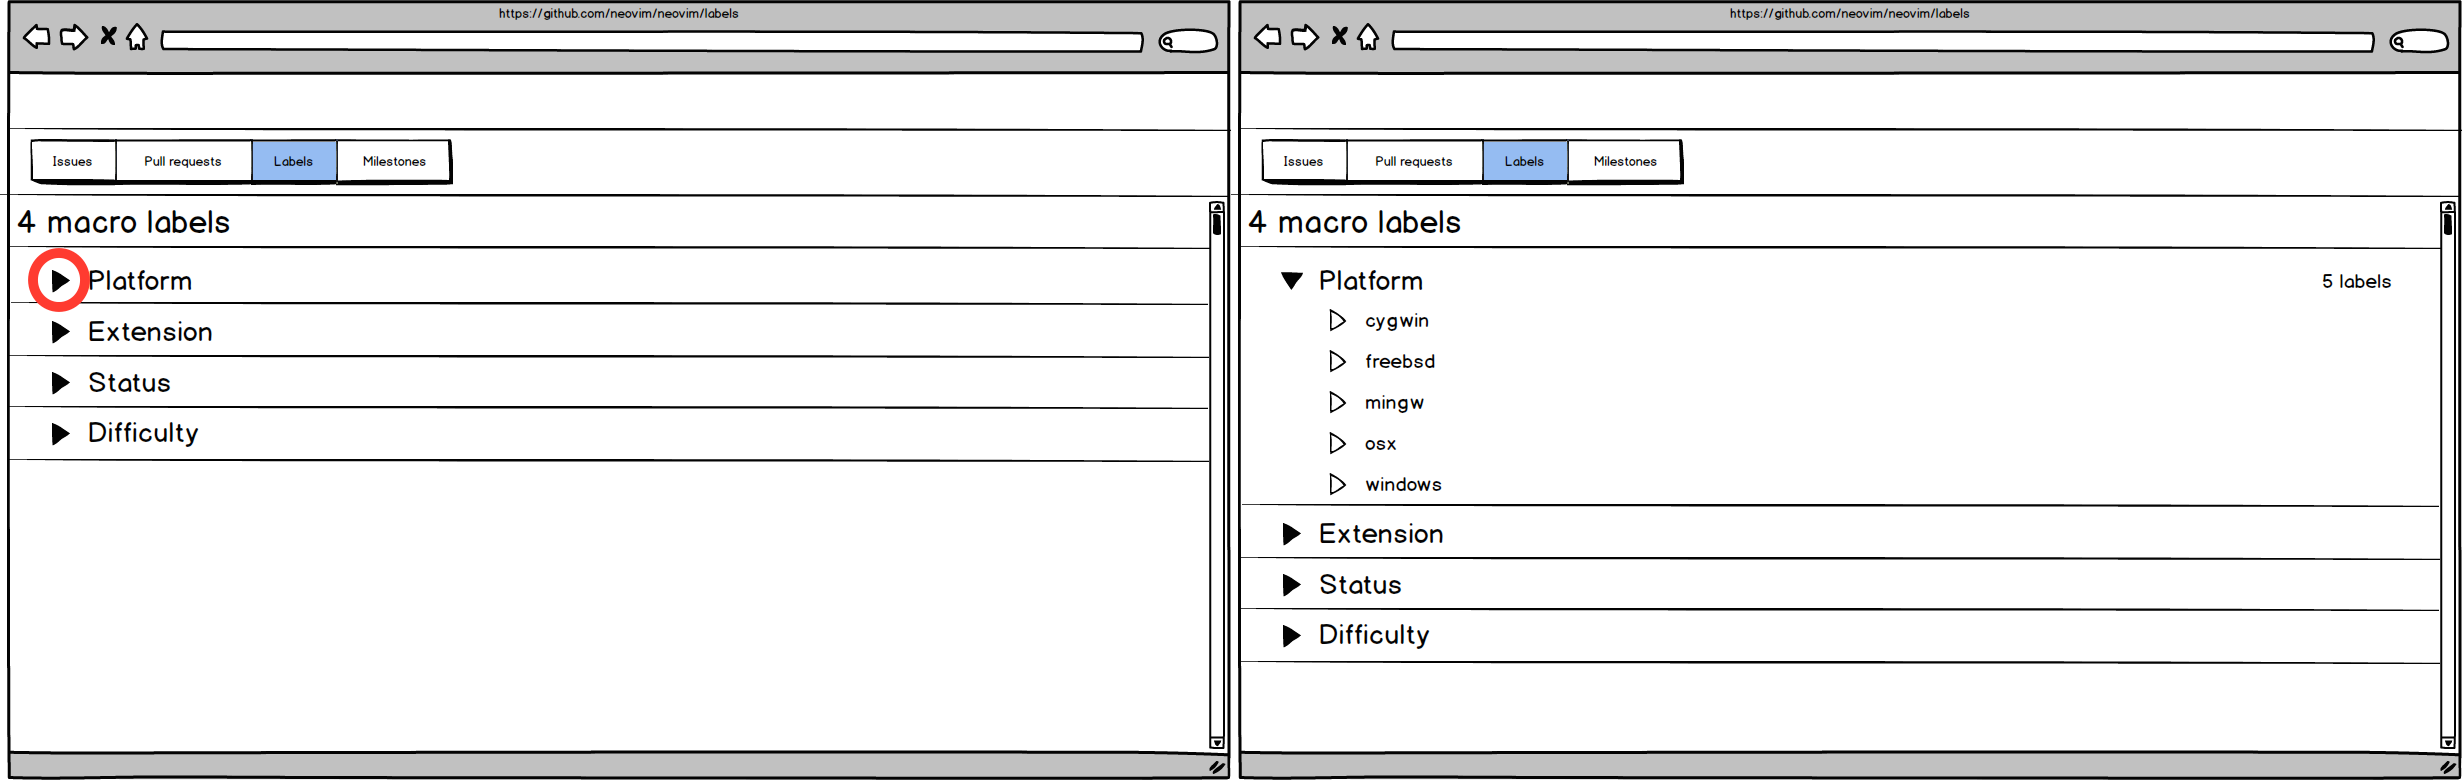
\includegraphics[width=0.9\linewidth]{low_prototype.png}}
\caption{Espansione di una macroarea.}
\label{fig:low_prototype}
\end{figure}

\subsubsection{Decisioni di design}
A seguito della discussione con componenti di altri gruppi durante l'ultimo workshop e, aver ricevuto dei feedback sul nostro prototipo iniziale, abbiamo deciso di seguire la linea iniziale, apportando per\`o le seguenti leggere modifiche:
\begin{itemize}
\item un \textbf{triangolo pieno} indica una macro-area che \`e possibile espandere (ovvero che contiene ulteriori labels).
\item un \textbf{triangolo vuoto} indica una macro-area che \emph{non} contiene nulla al suo interno; questo concetto pu\`o ripetersi sia al livello della macro-area che a quello delle labels annidate in una categoria pi\`u grande (Figura~\ref{fig:low_prototype}).
\item la scelta di una struttura \textbf{gerarchica} \`e nata dal fatto che chiunque abbia usato un gestore di file su un computer ha chiara l'idea di cartella, tramite la quale \`e possibile organizzare i propri dati in modo coerente. Questo ci permette di utilizzare un concetto non nuovo in un contesto diverso dal quale l'utente si aspetta di trovarlo, rendendo ragionevolmente immediato l'utilizzo della nostra funzionalit\`a.
\end{itemize}

\begin{figure}[H]
\center{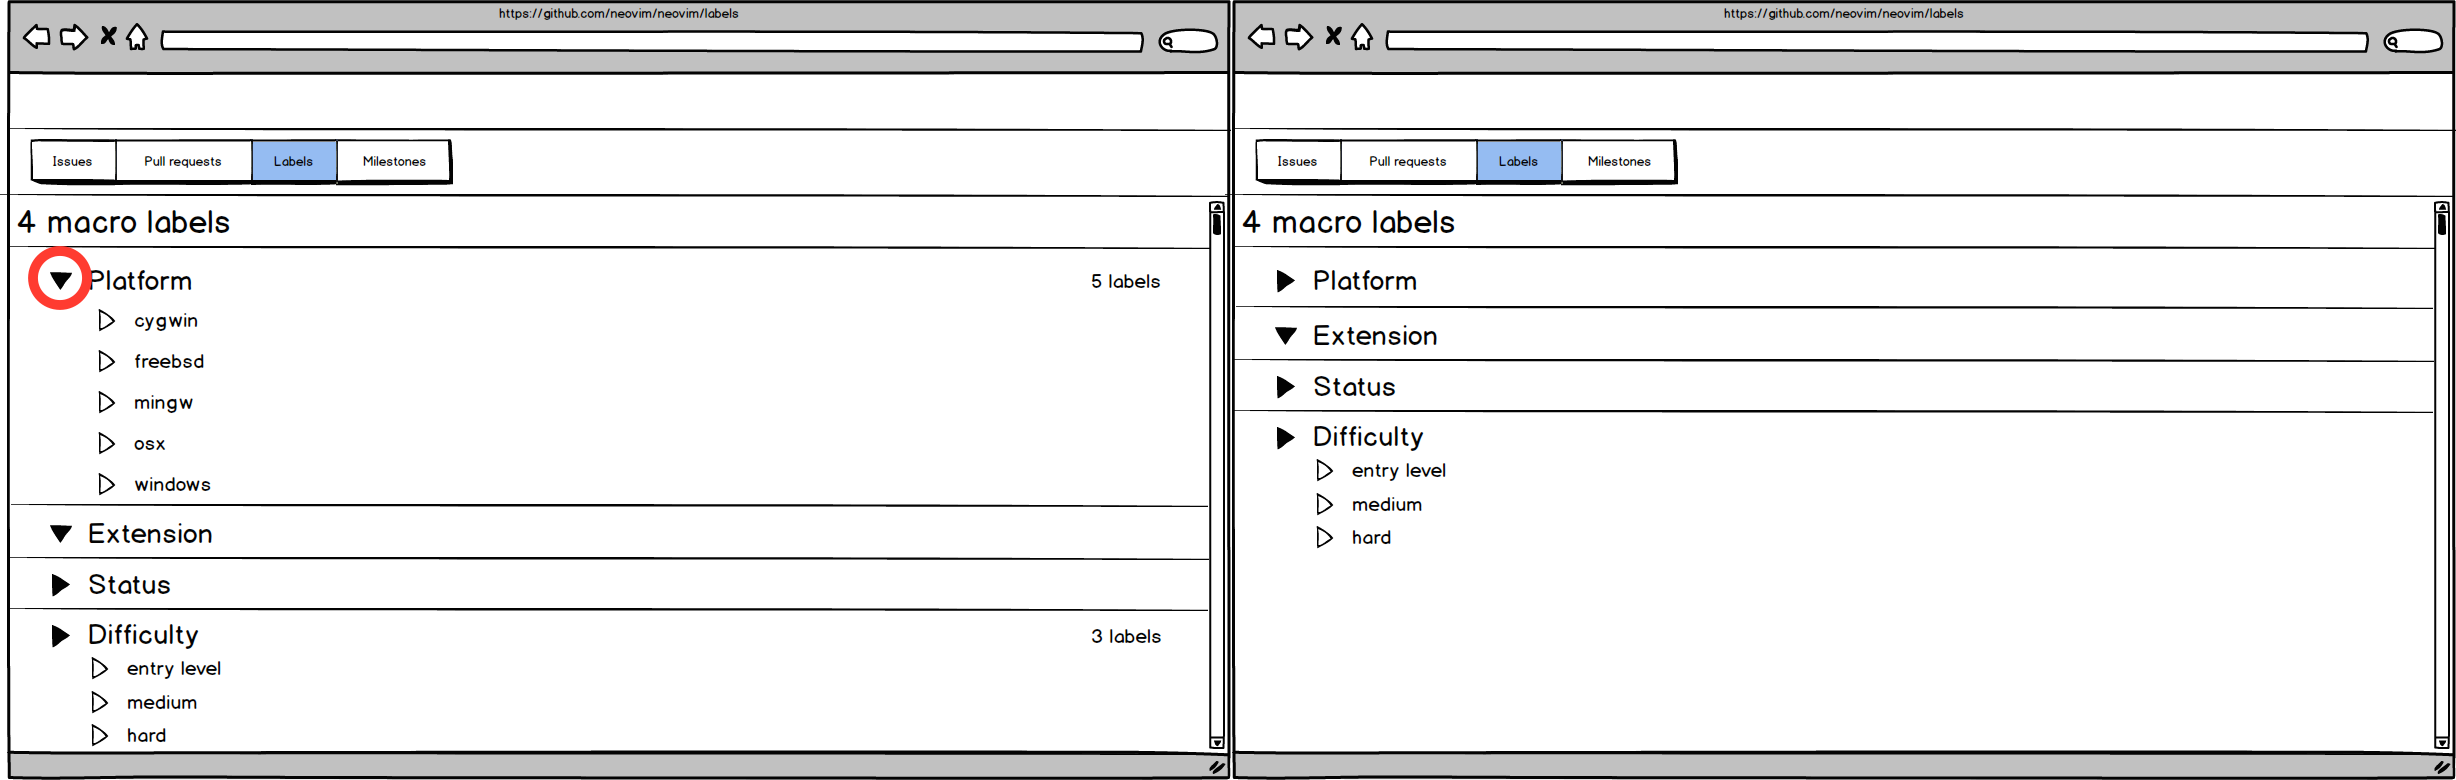
\includegraphics[width=0.9\linewidth]{low_prototype2.png}}
\caption{Struttura gerarchica delle etichette.}
\label{fig:low_prototype2}
\end{figure}

Dalla Figura~\ref{fig:low_prototype2} \`e possibile vedere come abbiamo realizzato il nostro prototipo a bassa fedelt\`a conclusivo.\\

\subsection{Prototipo ad alta fedelt\`a}
Abbiamo optato per l'\emph{implementazione} del prototipo ad alta fedelt\`a piuttosto che utilizzare dei tool che simulassero l'interattivit\`a per ottenere tutte le funzionalit\`a a cui puntavamo, senza penalizzare il \emph{look and feel} del prodotto finale~\cite[p.~263]{InteractionDesign}.\\
Ci\`o ci permette di avere un elaborato il pi\`u possibile interattivo\footnote{Non avendo alcun accesso alla parte di backend della piattaforma ma solamente alla parte di frontend, non ci \`e stato possibile renderlo completamente funzionante (eg.\ funzionalit\`a di aggiunta etichette, modifica label \dots)} che delinea con chiarezza il nostro obiettivo.\\
Dopo aver ricevuto alcuni feedback sul prototipo da parte di alcuni amici, abbiamo deciso di utilizzare le seguenti convenzioni:
\begin{itemize}
\item un \textbf{triangolo vuoto} contrassegna una macro-area espandibile
\item un'\textbf{etichetta} simboleggia una label annidata all'interno di una macro-area
\item un \textbf{diamante} indica una macro-area non ulteriormente espandibile (una categoria attualmente senza labels al suo interno)
\end{itemize}
Per permettere la gestione delle labels, sono stati aggiunti i bottoni \emph{new category} e \emph{add}, che permettono di aggiungere una macro-area alla lista ed una label annidata all'interno della categoria scelta rispettivamente.

\begin{figure}[H]
\center{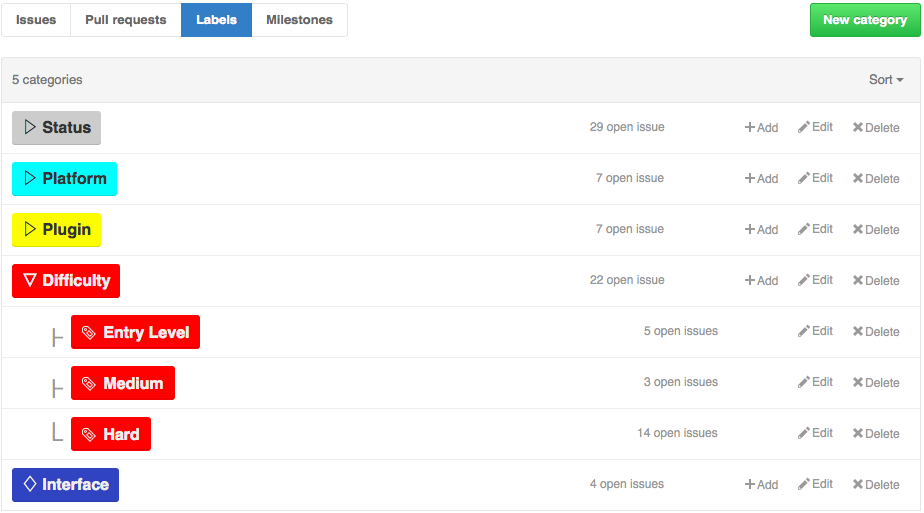
\includegraphics[width=0.55\linewidth]{dopo.png}}
\caption{Prototipo ad alta fedelt\`a definitivo.}
\label{fig:dopo}
\end{figure}

\subsubsection{Analisi dei colori}
Dopo aver utilizzato una struttura gerarchica per una visualizzazione pi\`u chiara ed intuitiva, abbiamo deciso di soffermarci anche sulla scelta dei \emph{colori} da assegnare alle etichette.\\
Ogni colore, che sia primario oppure secondario, viene percepito da ogni utente in modo diverso e personale: esso \`e fortemente legato all'esperienza e alla cultura di ognuno.\\
Il colore \emph{rosso}, ad esempio, nella cultura occidentale viene immediatamente e quasi inconsciamente associato ad un segnale di pericolo o ad un avvertimento che catturi l'attenzione. Nella cultura orientale, invece, simboleggia aspetti positivi della vita, come la fortuna e la gioia. Possiamo quindi capire come l'associazione colore-esperienza possa risultare estremamente diversa in presenza di contesti sociali differenti~\cite[p.~9-12]{thesis}.\\
Secondo questo principio, lasciare all'utente la scelta del colore delle labels permetterebbe una maggiore flessibilit\`a, ma al contempo si tornerebbe al problema descritto nel Paragrafo\ref{badexamples}.\\
Per risolvere questa problematica abbiamo deciso di optare per una palette di colori di default pi\`u ristretta.

\begin{figure}[H]
\center{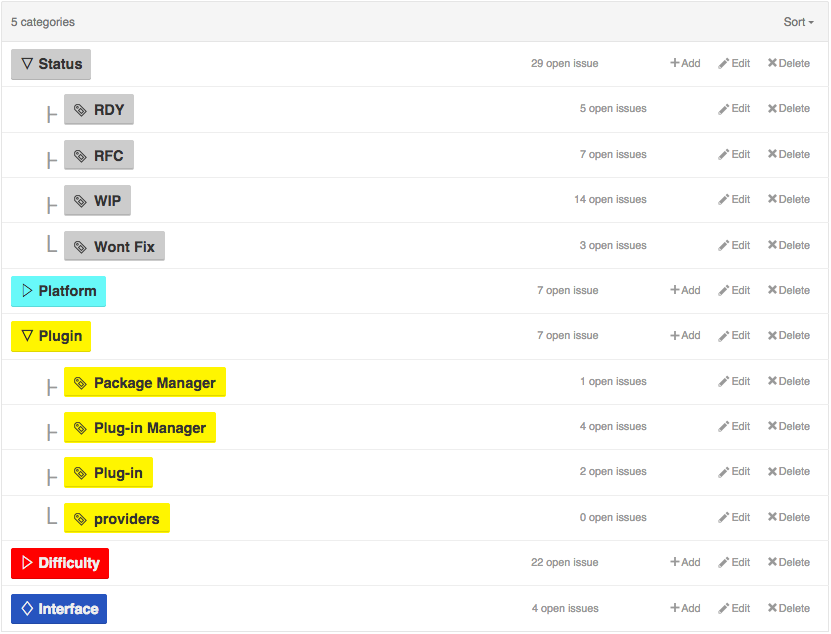
\includegraphics[width=0.6\linewidth]{finale.png}}
\caption{Utilizzo e scelta dei colori delle labels.}
\label{fig:finale}
\end{figure}

Come si pu\`o vedere dalla Figura~\ref{fig:finale}, la struttura ad albero \`e ben visibile sin da subito. I colori per questo prototipo sono stati scelti pensando anche a come questi vengono visti da una persona daltonica\footnote{\url{http://www.visibone.com/color/chart2x.html}}.\\
Dalla Figura~\ref{fig:daltonici}\footnote{\url{http://www.colormatters.com/color-and-vision/what-is-color-blindness}} \`e possibile notare come alcuni colori ben distinguibili per i soggetti normovisivi non lo siano affatto per chi \`e affetto da una forma di daltonismo.

\begin{figure}[H]
\center{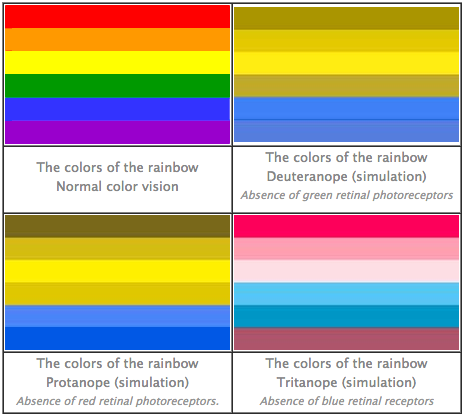
\includegraphics[width=0.45\linewidth]{paletteDaltonici.png}}
\caption{Comparazioni tra normovisivi e daltonici.}
\label{fig:daltonici}
\end{figure}

Alla luce di questo approfondimento, abbiamo optato per:
\begin{itemize}
\item il colore rosso per la categoria della difficolt\`a, perch\'e possa essere immediatamente identificabile e risalti rispetto al resto della pagina (come detto nel Paragrafo\ref{motivi}, non conoscere la complessit\`a delle issues \`e un grosso ostacolo alla partecipazione).
\item un colore neutro come il grigio per indicare lo stato di un task, dal momento che \`e un'informazione utile per tenere sotto controllo il flusso del lavoro, ma non risulta cos\`\i\ essenziale.
\item gli altri colori utilizzati sono stati scelti in modo che possano essere distinguibili da chiunque, in modo da non sacrificare l'accessibilit\`a della piattaforma.
\end{itemize}
L'idea di limitare la scelta di colori durante la creazione delle labels sacrifica la libert\`a dell'utente a favore di una interfaccia pi\`u accessibile e ben organizzata. Al tempo stesso la nostra implementazione fornisce gli strumenti necessari per gestire in modo consono le etichette: ci\`o non significa che la nostra impedisca all'utente finale di configurare i colori come meglio crede.

\newpage

\section{Considerazioni finali}
Dopo aver investito molto tempo in questo progetto ed aver accresciuto le nostre competenze, potrebbe risultare complicato valutare in modo obiettivo il lavoro da noi svolto.\\
I paragrafi seguenti si prefiggono di trarre delle valide ed oggettive conclusioni.

\subsection{Confronto con l'attuale implementazione}
Nella Figura~\ref{fig:confronto} si evince quanto la struttura da noi proposta aumenti l'usabilit\`a del prodotto anzich\'e fuorviare l'utente. Per fare ci\`o abbiamo sacrificato leggermente l'intuitivit\`a nell'immediato (eg.\ quando si deve aggiungere una label annidata) per aumentare la produttivit\`a sul lungo periodo. Questo comporta una drastica diminuzione del tempo impiegato per decifrare il reale significato delle labels.\\
Si noti come alcuni progetti, tra cui Neovim stesso, tenti di simulare questa struttura gerarchica componendo i nomi (eg.\ platform:cgwin, platform:freebsd, come da Figura~\ref{fig:cattivoesempio2}).

\begin{figure}[H]
\center{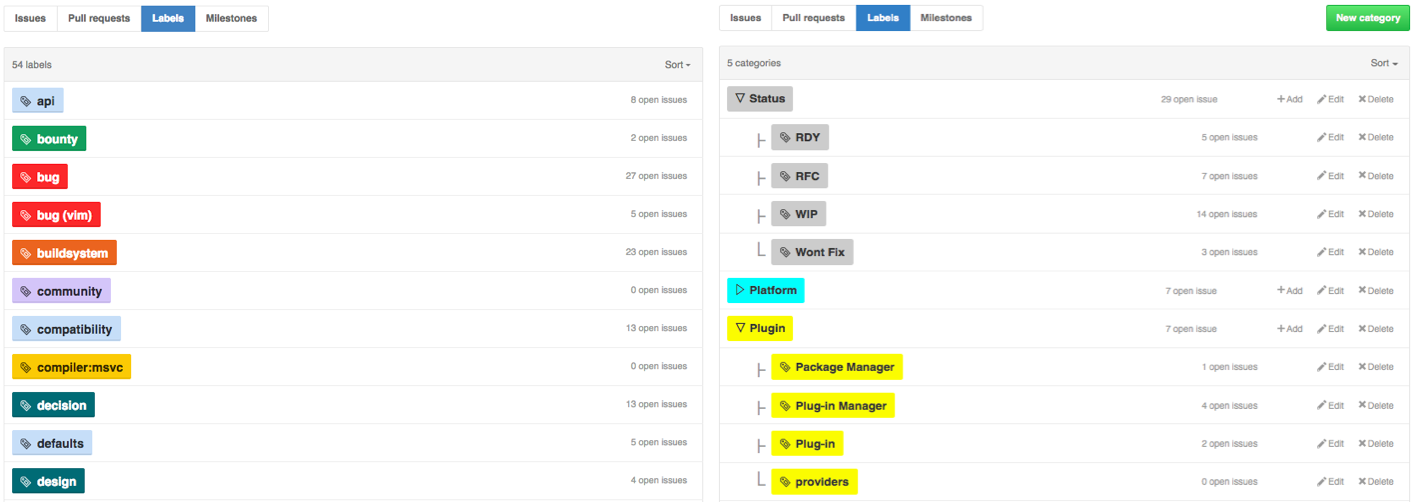
\includegraphics[width=0.8\linewidth]{confronto.png}}
\caption{A sinistra l'attuale implementazione, a destra la nostra proposta.}
\label{fig:confronto}
\end{figure}

Seguendo il metodo iterativo di \emph{(re) design-evaluation} che \`e possibile vedere in Figura~\ref{fig:ciclo}, abbiamo ottenuto un prototipo finale che \`e frutto di step incrementali, permettendoci cos\`\i\ di sfruttare non solo la nostra esperienza e capacit\`a critica, ma anche quella di altre persone che ci hanno riportato dei feedback dopo aver visionato il nostro lavoro.

\begin{figure}[H]
\center{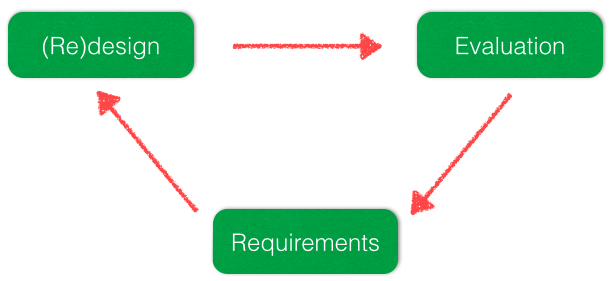
\includegraphics[width=0.45\linewidth]{cycle.png}}
\caption{Processo di design con iterazioni.}
\label{fig:ciclo}
\end{figure}

\subsection{Conclusione}
Dall'analisi delle risposte fornite dagli intervistati e dalla nostra esperienza possiamo affermare che la principale difficolt\`a nel contribuire a progetti open source sia causata dagli strumenti a disposizione dei team di sviluppo per la loro gestione. Tale ipotesi \`e stata confermata anche dal nostro studio su NeoVim durante il quale, infatti, non abbiamo riscontrato impedimenti rilevanti n\'e nella struttura n\'e nella gestione del progetto.\\
% #dash is right (shut up please syntastic).
GitHub \`e considerato lo stato dell'arte, ed il fatto che anche il team di sviluppo di GoLang\footnote{\url{https://groups.google.com/forum/#!topic/golang-dev/sckirqOWepg\%5B1-25-false\%5D}}, progetto Google, lo abbia preferito all'utilizzo di strumenti interni (Google Code\footnote{\url{https://code.google.com/}}) ne \`e dimostrazione.\\
Al termine di questo progetto ci samo resi conto che svolgerne alcune parti in modo differente e pi\`u approfondito avrebbe potuto portare a risultati pi\`u significativi.\\
Senza dubbio intervistare un maggior numero di persone, in particolare pi\`u sviluppatori, avrebbe potuto rendere maggiormente concreta la raccolta dei dati e dei requisiti, permettendoci in questo modo di delineare una \emph{personas} pi\`u accurata e di individuare ulteriori problematiche che potrebbero essere sfuggite alla nostra analisi.\\
I problemi principali che possono essere risolti tramite un redisign dell'interfaccia grafica (UI) sono quelli che dissuadono gli utenti pi\`u esperti dal collaborare. Bisogna comunque tenere presente che risulta poco verosimile pensare di poter coinvolgere persone senza un certo tipo di competenze ed \`e difficile avvicinare allo sviluppo di un progetto open source coloro che non vogliono per motivi ideologici.\\
Infine, date le tempistiche relativamente brevi, non \`e stato possibile entrare pi\`u nel dettaglio per quanto riguarda l'associazione dei colori alle labels e la relativa accessibilit\`a per individui affetti da daltonismo.

%bibliography: dev dirty hack
%\cite{*}

\newpage
\bibliographystyle{unsrt}
\bibliography{consegna_finale}

\end{document}
